% This is "sig-alternate.tex" V2.1 April 2013
% This file should be compiled with V2.5 of "sig-alternate.cls" May 2012
%
% This example file demonstrates the use of the 'sig-alternate.cls'
% V2.5 LaTeX2e document class file. It is for those submitting
% articles to ACM Conference Proceedings WHO DO NOT WISH TO
% STRICTLY ADHERE TO THE SIGS (PUBS-BOARD-ENDORSED) STYLE.
% The 'sig-alternate.cls' file will produce a similar-looking,
% albeit, 'tighter' paper resulting in, invariably, fewer pages.
%
% ----------------------------------------------------------------------------------------------------------------
% This .tex file (and associated .cls V2.5) produces:
%       1) The Permission Statement
%       2) The Conference (location) Info information
%       3) The Copyright Line with ACM data
%       4) NO page numbers
%
% as against the acm_proc_article-sp.cls file which
% DOES NOT produce 1) thru' 3) above.
%
% Using 'sig-alternate.cls' you have control, however, from within
% the source .tex file, over both the CopyrightYear
% (defaulted to 200X) and the ACM Copyright Data
% (defaulted to X-XXXXX-XX-X/XX/XX).
% e.g.
% \CopyrightYear{2007} will cause 2007 to appear in the copyright line.
% \crdata{0-12345-67-8/90/12} will cause 0-12345-67-8/90/12 to appear in the copyright line.
%
% ---------------------------------------------------------------------------------------------------------------
% This .tex source is an example which *does* use
% the .bib file (from which the .bbl file % is produced).
% REMEMBER HOWEVER: After having produced the .bbl file,
% and prior to final submission, you *NEED* to 'insert'
% your .bbl file into your source .tex file so as to provide
% ONE 'self-contained' source file.
%
% ================= IF YOU HAVE QUESTIONS =======================
% Questions regarding the SIGS styles, SIGS policies and
% procedures, Conferences etc. should be sent to
% Adrienne Griscti (griscti@acm.org)
%
% Technical questions _only_ to
% Gerald Murray (murray@hq.acm.org)
% ===============================================================
%
% For tracking purposes - this is V2.0 - May 2012

\documentclass{sig-alternate-05-2015}

\usepackage{amsmath,amsfonts}
\usepackage{times}
\usepackage{url}
\usepackage{color}
\usepackage{latexsym}
\usepackage{epsfig}
\usepackage{subfig}
\usepackage{graphicx}
%\usepackage[pdftex]{graphicx}
%\DeclareGraphicsExtensions{.pdf,.jpeg,.png}
%\usepackage{epstopdf}
\usepackage{booktabs}
\usepackage{diagbox}
\usepackage{array}
\usepackage{multicol}
\usepackage{threeparttable}

\newcommand{\figref}[1]{Figure \ref{#1}}
\newcommand{\tabref}[1]{Table \ref{#1}}

\newcolumntype{I}{!{\vrule width 1pt}}
\newlength\savedwidth
\newcommand\whline{\noalign{\global\savedwidth\arrayrulewidth
                            \global\arrayrulewidth 1pt}%
                   \hline
                   \noalign{\global\arrayrulewidth\savedwidth}}
\newlength{\Oldarrayrulewidth}
\newcommand{\Cline}[2]{%
  \noalign{\global\setlength{\Oldarrayrulewidth}{\arrayrulewidth}}%
  \noalign{\global\setlength{\arrayrulewidth}{#1}}\cline{#2}%
  \noalign{\global\setlength{\arrayrulewidth}{\Oldarrayrulewidth}}}

\newcommand\norm[1]{\left\lVert#1\right\rVert}
\DeclareMathOperator*{\argmin}{arg\,min}

\newcommand{\KZ}[1]{\textcolor{blue}{Kenny: #1}}
\newcommand{\YZ}[1]{\textcolor{yellow}{Yizhong: #1}}


\begin{document}

% Copyright
%\setcopyright{acmcopyright}
%\setcopyright{acmlicensed}
%\setcopyright{rightsretained}
%\setcopyright{usgov}
%\setcopyright{usgovmixed}
%\setcopyright{cagov}
%\setcopyright{cagovmixed}

% DOI
\doi{}

% ISBN
\isbn{}

%Conference
%\conferenceinfo{PLDI '13}{June 16--19, 2013, Seattle, WA, USA}

%\acmPrice{\$15.00}

\title{Mining Word Semantic
Difference between American and British English}

\maketitle
\begin{abstract}
This paper presents an initial attempt to automatically discover
English words that have different semantics between British and
American uses from a large collection of English literature.
We compare several purely data-driven, unsupervised approaches
and conclude that modeling words by their embeddings using the skip-gram
model outperforms the other baseline methods, and achieves a 0.247 F1@1000,
57.3\% more than the simpler TF-IDF method.
This study will benefit linguists, language educators and learners, especially
when it comes to new English words not yet included in dictionaries.
\end{abstract}


%
% The code below should be generated by the tool at
% http://dl.acm.org/ccs.cfm
% Please copy and paste the code instead of the example below.

\category{I.2.7}{Natural Language Processing}{Text analysis}
\category{I.7.5}{Document Capture}{Document analysis}
\category{H.2.8}{Database Applications}{Data mining}
\category{H.3.1}{Content Analysis and Indexing}{Linguistic processing}

%
% End generated code
%

%
%  Use this command to print the description
%
\printccsdesc

% We no longer use \terms command
%\terms{Theory}

\keywords{natural language processing; word embedding; semantic difference}

\section{Introduction}

Protein$-$protein interactions (PPIs) are of central importance for the majority of biological functions, such as signal transduction, metabolic pathways, molecular dynamics, and protein networks\cite{Hoffmann.Krallinger.ea:2005}, for they serve as the most fundamental building blocks of the entire interacademic systems of any organisms. Collecting data on pairwise interaction relationships is essential for multiple purpose, including identification of modules with certain functionality\cite{Spirin.Mirny.03}, mapping diseases to dominated genes\cite{Ideker.Sharan.08}, and after all, understanding wholistic metabolic/genetic networks from a system biology perspective.

A lot of databases have been built to store protein and genetic interactions from major model organism species and are available in various standardized formats, such as MINT\cite{Zanzoni.Montecchi-Palazzi.ea:2002}, BIND\cite{Bader.ea:2003}, BIOGRID\cite{DBLP:journals/nar/StarkBRBBT06}, etc. Among those mainstream databases, the data largely rely on voluntary reports by scientists or researchers, besides, comprehensive curation efforts become indispensable for the sake of accuracy. However, the amount of biology-related literatures with respect to protein interactions grows explosively and thus make it either impossible or impractical to manually detect PPI information anymore.

Considering huge amount of PPI information with great wealth hidden in published papers, in recent years, numerous mining techniques have been proposed that aim to extract PPI information automatically from free text, especially machine learning, information retrieval, and natural language processing\cite{DBLP:journals/bib/WinnenburgWPDS08}.These approaches can be roughly categorized into three classes: co$-$occurrence, rule$-$based, and machine learning. 

Co$-$occurrence is the approach with most simplicity and naivete. Just as its name implies, this method intends to find out pairs of proteins that co-occur in the same context. The scope of "same context" ranges from phrase, sentence, paragraph to whole abstract, even document. The underlying assumption is that whenever two proteins are mentioned together by authors, chances are high that there is some kind of relationship between them. However, however, in-context closeness even semantic relation does not necessarily represent actual biological interaction. As a consequence, a large fraction of candidate pairs are mismatched inevitably, causing a high recall but low precision.

The second approach is rule-based extraction, in other words, pattern matching. There are many types of rules, most of them concern natural language processing (NLP). One way is to specify hand-crafted regular expressions before hand, which mostly lean on language usage preference. Besides, by using full or partial (shallow) parsing strategies, more information would be acquired, such as part-of-speech taggers, local dependencies between syntactic components, context-free grammar\cite{DBLP:journals/bioinformatics/TemkinG03}, and full sentence structure. Compared to co$-$occurrence, rule-based approach enjoy better precision but much lower recall. In addition, since the rules are usually derived from training data, that is to say, the improper choice of training data would be significantly lethal, therefore quality of extraction is invariably instable and may not applicable to other data.

The third and most commonly used approach use machine learning techniques, in this case, the task to extract protein$-$protein interactions turns out to be a binary classification problem. Each protein pairs are represented along with a set of features, which is associated with their context, then a well$-$defined classifier gives the answer whether the candidate protein pairs is classified to be qualified PPI. (TO BE FURTHER FILLED!!!)

In this paper, we introduce a general bootstrapping framework for Protein$-$protein interaction extraction from natural text.Our method differs from most of the previous works in three aspects:

(1)The extraction process is driven by only tiny fraction of training data, which are regarded as seed data. In each round, it would derive reliable patterns automatically from seed data, then extract more positive PPI pairs consequently, what's more, the seed data would be augmented by the newly extracted results with high confidence.

(2)multiple graph kernel. 

(3)various evaluation.





\section{Approach}
\label{sec:approach}
In this section, we first introduce the general framework of ChatMatch, which is modeled as
a sport tournament, then discuss some possible scoring functions that can be used by
the virtual judges in these competitions.

%Our whole evaluation framework consists of competition and scoring at three different levels. 
%The game level is at the bottom 
%and is played between two players. 
%Then comes the match level.
%To ensure the fairness of the game, 
%two games will be played between every two robots, 
%with each side starting a conversation.
%The result of two games determines the outcome of a match. 
%The tournament level is at the top
% and is composed of matches among different pairs of players. 

\subsection{Competition Protocol}
\label{sec:competition}
The competition takes place, from top to bottom, at tournament, match and
game levels.

\subsection*{Tournament Rules}
%\KZ{Give an overview of the how the tournament is run.}
We adopt a double round-robin 
sports tournament, where all bots participating in the competition 
converse directly with each other twice.
This is better than a knock-out system because it assesses a bot's ability to
deal with both strong and weak bots.
%For example, whether with weaker bots will induce them to make more mistakes or  how stronger bots will motivate their performance.
If we have $n$ chatbots players in our tournament, 
there will be $n\times (n-1) $ games in total.

\subsection*{Match Rules}
%\KZ{Talk about how the matches are administered. Just the procedure only.}
There are two chatbots competing in a single match. 
Each match consists of two games,
 started by a different bot. 
If we have $n$ bots in our tournaments, there 
will be ${n \choose 2}$ matches in total. 

\subsection*{Game Rules}
%\KZ{The procedure of the game. How each game is started and stopped.}
Each game is started by a player whose first utterance is provided by 
the system. The choice of the first utterance can be different 
depending on the domain of the bots and the ability we want to 
rank about the bots. For example, if we want to test 
the ability on movies, we can set a movie-related 
first utterance. 

During a game, there might be different ways to 
end the conversation. We can set a fixed number of exchanges 
or a terminating condition such as whether a bot makes a fatal error
or whether a certain score is reached.

\begin{table*}[th]
\centering
\scriptsize
\begin{tabular}{c|l|l}
%\hline
\toprule
\textbf{Dimension} & \textbf{Definition} &\textbf{Approach} \\ \midrule
Fluency  & Responses are fluent and natural.& Sentence perplexity. \\
Knowledge & Responses indicate the bot has the knowledge. & The number of times the bot expresses its ignorance to a question.\\
Proactivity & Responses actively proceed the conversation.&The number of times the bot raises a question. \\
Specificity & Responses are not generic.&The average of Distinct-1 and Distinct-2 \citep{li2015diversity}.\\
Diversity &Responses which are diverse and non-repetitive. &Repetition detection following the function in \algoref{algo:rep}. \\
Consistency &Responses do not contradict chat history. &Detect inconsistent questions following the function in \algoref{algo:inconsist}\\
Relevance & Responses are related to current context.& Ability to catch the relevant concept in chat history defined in \algoref{algo:bonus}. \\
\bottomrule
\end{tabular}
\caption{Seven evaluation dimensions.}
\label{tab:methods}
\end{table*}


\subsection{Scoring}
\label{sec:scoring}
\subsection*{Game-level Scoring}
%\KZ{Define a few functions: one to catch repeating, one to chat contradiction and one to catch long term memory.}

%Here we define the rules for recording points in one game between two bots. 
Inspired by \citet{finch2020towards}, 
we score each turn based on seven aspects of rules 
concerning \textit{consistency}, \textit{fluency}, \textit{knowledge}, \textit{specificity}, 
\textit{diversity}, \textit{relevance} and \textit{proactivity}. 
%As these seven metrics present a high level of 
%overlap among all distinct evaluation metrics used 
%during different process of human evaluation,
%we believe the combination of these seven distinct dimensions will be reliable. 
Finally, we sum up the scores for each bot for all the turns.
\tabref{tab:methods} documents the definition of these dimensions, which can all be scored
automatically.

%After finishing the calculation of the bonus and penalty scores for each turn, we obtain the scores of the two bots in a game with weighted sum according to \eqnref{eq:sum-up}

%\begin{equation}
%S(bot) = \sum_t - c\times C(t)  - r \times R(t) + b \times B(t)
%\label{eq:sum-up}
%\end{equation}
%$S$ denotes the total score gained by a bot for a game.
\begin{figure}[th]
        \centering
        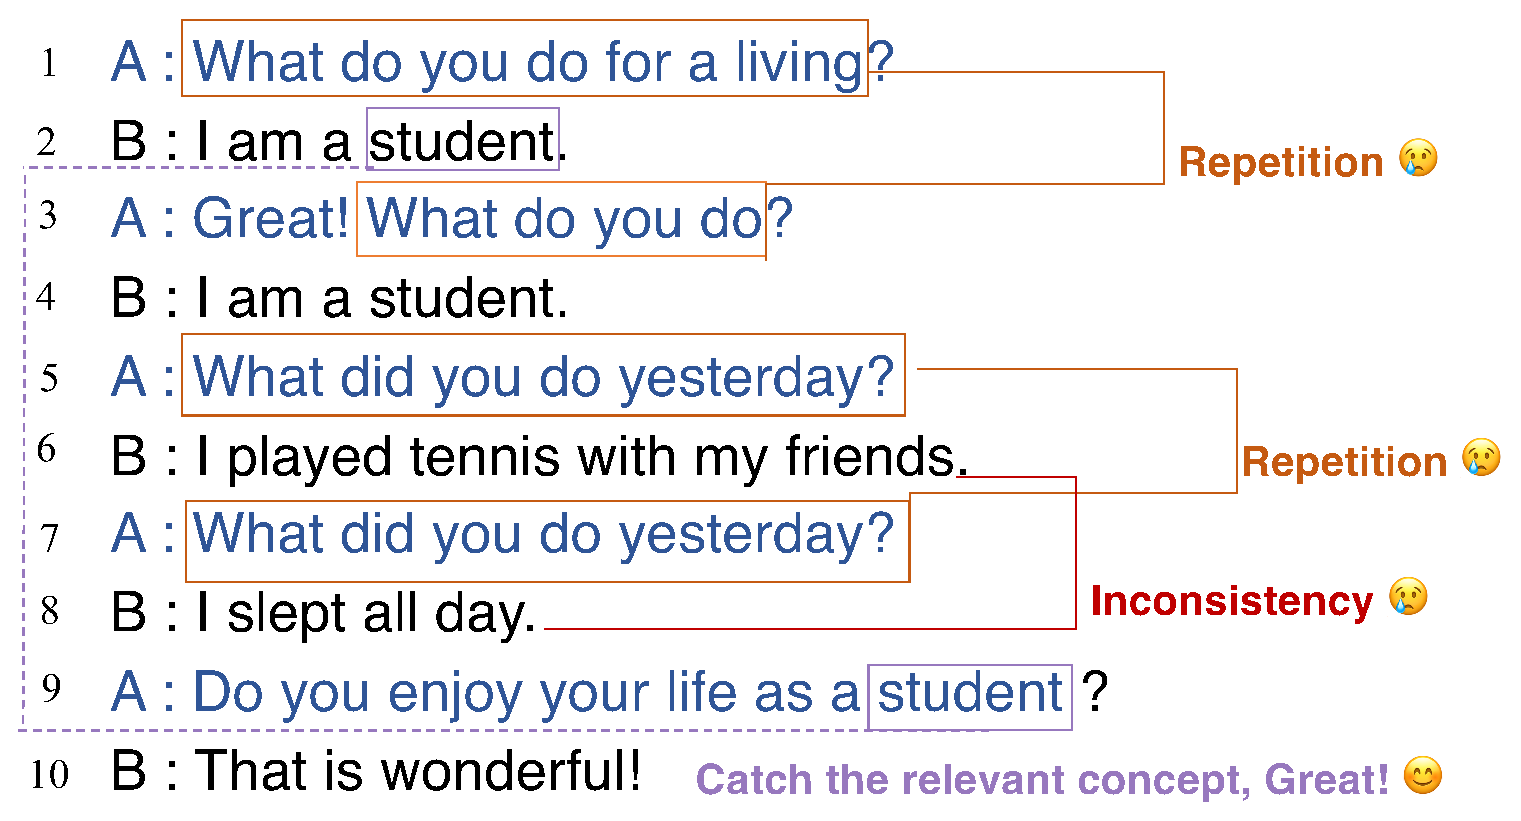
\includegraphics[width=0.95\columnwidth]{example2.eps}
        \caption{A chat snippet between two bots.}
        \label{fig:example}
\end{figure}

Fluency, Knowledge, Proactivity and Specificity are scored for each turn separately
and aggregated at the end of the conversation.
Detection for diversity, consistency and relevance are more involved and are explained
using \figref{fig:example}. 

As for diversity, at each turn $t$, we first check if there exists any repetitive question.  
We can easily find turn 3 and turn 7 repeated turn 1 and turn 5 
respectively. They will then be penalized one point for repetition. 
Repetition is not penalized if the previous turn is already 
marked as a repetitive question. For example, in \figref{fig:example}, 
although turn 4 is considered a repetition of turn 2,  
we are not going to penalize it as turn 3 is a repetitive question. 

The detection of inconsistency is always triggered after the detection of repeated questions. 
If the answers to the same questions are different, we will penalize the current turn, 
such as turn 8 in \figref{fig:example}.

We decide a repetition or an inconsistency by calculating the similarity of the two turns. 
We use a similarity function to complete the calculations, which we will 
discuss in \secref{sec:experiment}. The actual diversity and consistency scores
are the negation from the amount of repetition and inconsistency.

Relevance is assessed as a bonus to reward
a bot if it is able to memorize the important relevant concepts that have shown up 
before in the conversation. We sort the concepts that have shown up in 
chat history by their IDF scores. For example, in turn 9, $A$ 
mentions the concept word ``student'' presented by $B$ in turn 2. With this
turn, $A$ will win a bonus point.


The algorithms and notations for computing diviersty, consistency and relevance are included
in \tabref{tab:functions}, \algoref{algo:rep}, \algoref{algo:inconsist}, and \algoref{algo:bonus}. 

\begin{table}[th]
\centering
\small
\begin{tabular}{c|l}
%\hline
\toprule
\textbf{Notation} & \textbf{Description} \\ \midrule
$t$ & Current turn \\
$H(t)$  &  a list of history turns prior to $t$ \\
$Sim(x,y)$ & similarity between two turns $x$ and $y$ \\
$\sigma_r$ & Threshold for detecting repetition \\
$\sigma_c$ & Threshold for detecting consistency \\
$r$ & Weight for repetition \\
$c$ & Weight for inconsistency \\
$b$ & Weight for bonus \\
$d$ & Min distance between consecutive mentions \\
IDF list & List of lemma in chatlog sorted by IDF\\
$p$ & Percentage of important lemmas in IDF list\\
$R(t)$ &  Repetition penalty for turn $t$ \\
$C(t)$ &  Inconsistency penalty for turn $t$ \\ 
$B(t)$ &  Memory bonus for turn $t$ \\
$Rep(t)$ & A list of repeated turns for turn $t$ \\  
\bottomrule
\end{tabular}
\caption{
Functions and variables in algorithms.}
\label{tab:functions}
\end{table}

\begin{algorithm}[th]
\small
\caption{Scoring for Diversity}
\label{algo:rep}
\hspace*{0.02in} {\bf Input:}
 $t$, $H$, $Sim$, $\sigma_{r}$
; \hspace*{0.02in} {\bf Output: } 
 $R$;
\begin{algorithmic}[1]
\State //Starting to detect repetition
\For {$u$ in $H(t)$}
	\If {$Sim(t,u) \geq \sigma_{r}$}
		\State Add $u$ to $Rep(t)$
	\EndIf
\EndFor
    \If{$len(Rep(t))\geq 0$}
        \If{$t$ is a question and We can find a question in $Rep(t)$}
        \State $ R(t) \leftarrow  R(t) + 1$ 
        \Else
        \If {the previous turn of $t$ is not a repetitive question}
        \State $R(t)) \leftarrow R(t) + 1$ 
        \EndIf
        \EndIf
    \EndIf
\end{algorithmic}
\end{algorithm}


\begin{algorithm}[th]
\small
\caption{Scoring for Consistency}
\label{algo:inconsist}
\hspace*{0.02in} {\bf Input:}
$t$, $H$, $Sim$, $\sigma_{c}$
; \hspace*{0.02in} {\bf Output:  } 
 $C$;
\begin{algorithmic}[1]
\State // Inconsistency detection
 \If {previous turn of $p$ is a repetitive question} 
   \If{ the response $res$ to the question repeated by turn $p$ contradicts turn $i$ with $Sim(t, res) \leq \sigma_{c}$ }
    \State $C(t) \leftarrow C(t) + 1$
   \EndIf
  \EndIf
\end{algorithmic}
\end{algorithm}

\begin{algorithm}[th]
\small
\caption{Scoring for Relevance}
\label{algo:bonus}
\hspace*{0.02in} {\bf Input:}
$t$, $p$, $d$
; \hspace*{0.02in} {\bf Output:  } 
$B$;
\begin{algorithmic}[1]
\State // Assessing the ability of catching relevant concepts\\
$B(t) \leftarrow 0$
\For {all tokens $tk$ in current turn $t$}
 \If {$t$ - previous occurrence turn of $tk > d$ and $tk$ in the top $p\%$ of the IDF list of all tokens in the dialogue} 
   \State $B(t) \leftarrow 1$
  \EndIf
 \EndFor
\end{algorithmic}
\end{algorithm}

At the end of each game, each bot gets seven scores, one for each dimension.  
After pairwise comparison on individual dimension, a bot gains one point for win and zero point for a tie or lose.
The final score of each bot is determined by the sum of their individual scores.
%\KZ{Are these scores positive or negative? Comparable between bots?}

\subsubsection*{Match-level Scoring}
%\KZ{Use an equation to compute the final scores?}
One match which consists of two games, each started with a different bot, 
decides winning or losing between two bots.
For match-level scoring, we mimic the scoring rules of soccer tournament. 
For each match, $W$ points for the winner,  
$T$ points for a tie and 
$L$ points for the loser.
The value of $W$, $T$ and $L$ will be discussed in \secref{sec:ablation}. 

%\KZ{At the match level, we need to consider different starting context for the bots? I think we should present a few options for the reader and say that we are limited to these.}

\subsubsection*{Tournament-level Scoring}
%\KZ{Use an equation to compute the final scores?}
We count the points by simply summing up their scores gained in every match. Currently, several bots with the same final rank are tolerated. For future study, it's possible to mimic more detailed rules presented in sports match such as determine their ranking based on their win-loss relationship in the match between them.  
If they are still tied, we could propose an “overtime” for these two bots, one human judge may observe their performance and then make the decision of the game.


\section{Evaluation}
\label{sec:evaluation}
Through the above approach, we translate two popular English knowledge graphs: \con and \pro into \zhcon and \zhpro, respectively. In terms of the word embedding, we use the Chinese Wikipedia dump on Aug 1, 2018,  to train word embedding with Word2Vec, where the vocabulary size is 110,978 and the embedding dimension is 300.\footnote{\url{https://code.google.com/archive/p/word2vec/}}
In this section, we evaluate the coverage and accuracy of \zhcon and \zhpro, respectively. The baseline experiment we choose is the direct translation using the translator, and we will denote it as \textbf{DT} later. For example, in the baseline, we translate triple (``ball'', AtLocation, ``ballroom'') by feeding ``ball, ballroom'' into translator, and split the translation result ``球, 舞厅'' into (``球'', AtLocation, ``舞厅'') as the final translation result. Here, we do not provide the translator with the contextualized sentence such as ``the ball is at the ballroom.'', since there are no fixed patterns in the translated sentence, which makes it hard to extract the corresponding part, even for the translated results of one particular relation.\footnote{For example, although ``french chefs are capable of preparing food.'' and ``spider web is capable of catching morning dew.'' share the same structure in English, they will be translated into ``法国厨师有能力准备食物。'' and ``蜘蛛网能够吸引晨露。'' respectively, which requires more than one pattern to split the translation result.}

%\KZ{In addition to the end-to-end eval on the two translated KBs, you also
%need to do some ablation tests. For example, what if you don't do the revision?
%Is there any alternative ways to do revision? You need to show that your way of
%revision is better than straightforward methods.}

\subsection{\zhcon}
\zhcon is a mixed Chinese common sense knowledge graph, which comes from two sources, 
the original Chinese part of \con and the translation result of the English part of \con.

\textbf{Coverage.}
As shown in Table \ref{tab:zh_conceptnet_coverage}, the size of \zhcon is \textbf{4.76} times as large as the original Chinese part of \con, 
which is a substantial increase in quantity. The size of \zhpro is not as 4.91 times as we expected, since there exists overlap in the process of merging.
To our best knowledge, there are no other Chinese knowledge graphs dedicated to common sense, and \zhcon will be the first large one with about 2 million edges, which, we hope, could be a valuable asset for Chinese common sense research.
\begin{table}[ht]
\caption{Size of \zhcon.}
\label{tab:zh_conceptnet_coverage}
\centering
\begin{tabular}{ll}\hline 
\textbf{Dataset}&\textbf{Size}\\\hline
1. Original Chinese Part in \con &438,307(x1.00)\\  
2. Translated English part in \con &1,716,327(x3.91)\\
\zhcon (Merge 1 and 2)&\textbf{2,085,681(x4.76}) \\\hline
\end{tabular}
\end{table}

\textbf{Accuracy.}
To evaluate the quality of \zhcon, 
we randomly sample 500 samples from original Chinese part in \con, 
\text{DT} result of English part in \con, translation result of English part in \con based on our two-steps approach (we denote it as \textbf{OURS} later), and \zhcon (which merges the Chinese part in \con and translated English part in \con of \textbf{OURS}), respectively. 
We ask two annotators to evaluate these samples. 
As Table \ref{tab:conceptnet_accuracy} shows, there exists 1\% error in the original Chinese part of \con, which comes from crowdsourcing errors.
%Since approximately 86\% of the data in \con comes from collaborative datasets, such as Wiktionary, DBpedia, etc 
Compared with the direct translation (\text{DT}), the accuracy of the translation result based on \textbf{OURS} has a relative gain of \textbf{2.8\%}.
The accuracy of \zhcon has also been improved to \textbf{89.6\%} due to the high quality of the merged original Chinese part from \con.

\begin{table}[ht]
\caption{Accuracy of different approaches. The Kappa coefficients \cite{landis1977measurement} of two annotators suggest a substantial agreement.}
\label{tab:conceptnet_accuracy}
\centering
\begin{tabular}{ll}\hline
	Approach & Accuracy (Kappa) \\ \hline
	1. Original Chinese part in Conceptnet& 98.3\%(0.58) \\
	2. \textbf{DT} of English part                 & 84.5\%(0.85) \\
	3. \textbf{OURS} & 87.3\%(0.85) \\
	Zh-Conceptnet (Merge 1 and 3) & \textbf{89.6\%(0.79)} \\\hline
\end{tabular}
\end{table}

\textbf{Qualitative Results.}
Our approach can handle some intractable word sense disambiguations, such as ``date'', ``ball'', ``court'', ``capital'', ``fan'', etc, as shown in the blue part in Table \ref{tab:zh_conceptnet_case}.
Besides, our method can translate (``fan'', RelatedTo, ``sector'') into (``扇'', RelatedTo, ``扇形''), while the result of \textbf{DT} is (``粉丝'', RelatedTo, ``部门''). This shows that our approach can disambiguate ``fan''  and ``sector'' at the same time. As for the errors in \zhcon, according to our observations, most errors in \zhcon come from the triples with the relation of ``RelatedTo''. Since the relation of ``RelatedTo'' is relatively weak in English such as (``blunt'', RelatedTo, ``money''), it becomes even weaker after translation, and the triples with the relation of ``RelatedTo'' account for 48.16\% of all the triples in \con. The red part in Table \ref{tab:zh_conceptnet_case} shows more error cases. 


\begin{table}[!htbp]
\caption{Some examples triples in \zhcon. Correct translations are in {\color{blue} blue}, and incorrect ones are in {\color{red}red}.}
\label{tab:zh_conceptnet_case}
\resizebox{\linewidth}{!}{%
\begin{tabular}{lll}\hline
	\textbf{English}                 & \textbf{OURS}     & \textbf{DT}  \\\hline
	{\color{blue}(date, fruit)/IsA}                  & {\color{blue}枣, 水果}     & {\color{blue}时间, 水果}    \\ 
	{\color{blue}(ball, ballroom)/AtLocation}        & {\color{blue}舞会, 舞厅}    & {\color{blue}球, 舞厅}     \\ 
	{\color{blue}(can, shelf)/AtLocation}            & {\color{blue}罐头, 货架}    & {\color{blue}可以, 货架}    \\ 
	{\color{blue}(court, gymnasium)/AtLocation}       & {\color{blue}球场, 体育馆}   & {\color{blue}法院, 体育馆}   \\ 
	{\color{blue}(munition, arm)/MannerOf}            & {\color{blue}军火, 武装}    & {\color{blue}军火, 手臂}    \\ 
	{\color{blue}(capital, proper noun)/AtLocation} & {\color{blue}大写, 专有名词}  & {\color{blue}资本, 专有名词}  \\ 
	{\color{blue}(spinach, can)/RelatedTo}             & {\color{blue}菠菜, 罐头}    & {\color{blue}菠菜, 可以}    \\ 
	{\color{blue}(fan, blow)/RelatedTo}             & {\color{blue}扇子, 吹}    & {\color{blue}粉丝, 吹}    \\ 
	{\color{blue}(fan, peacock)/RelatedTo}             & {\color{blue}扇子, 孔雀}    & {\color{blue}粉丝, 孔雀}    \\ 
	{\color{blue}(fan, sector)/RelatedTo}             & {\color{blue}扇, 扇形}    & {\color{blue}粉丝, 部门}    \\ 
	{\color{blue}(collection, garage)/AtLocation}             & {\color{blue}珍藏, 车库}    & {\color{blue}集合, 车库}    \\ 
	{\color{blue}(brook, tolerate)/RelatedTo}             & {\color{blue}容忍, 姑息}    & {\color{blue}小溪, 容忍}    \\ 
	{\color{red} (blunt, money)/RelatedTo}             & {\color{red} 生硬, 钱}    & {\color{red} 生硬, 钱}    \\ 
	{\color{red} (fouta, thin)/RelatedTo}             & {\color{red}伏塔加, 瘦}    & {\color{red}富塔, 瘦}    \\ 
	{\color{red}(major ninth, interval)/RelatedTo}             & {\color{red}主要的第九, 间隙}    & {\color{red}主要的第九, 间隔}    \\ 
	{\color{red}(melo, music)/RelatedTo}             & {\color{red}甜瓜, 音乐}    & {\color{red}melo, 音乐}    \\ \hline
\end{tabular}}
\end{table}

%粉丝    /r/RelatedTo    打击
%fan     ['球迷', '迷', '风扇', '扇子', '扇', '粉丝']
%blow    ['打击', '吹', '刮']
%扇子    吹      0.29190982571468305
%(fan, blow)/RelatedTo             & 扇子, 吹    & 粉丝, 吹    \\ \hline
%
%粉丝    /r/RelatedTo    孔雀
%fan     ['球迷', '迷', '风扇', '扇子', '扇', '粉丝']
%peacock ['孔雀']
%扇子    孔雀    0.2387474142191117
%(fan, peacock)/RelatedTo             & 扇子, 孔雀    & 粉丝, 孔雀    \\ \hline
%
%粉丝    /r/RelatedTo    部门
%fan     ['球迷', '迷', '风扇', '扇子', '扇', '粉丝']
%sector  ['扇形', '部门']
%扇      扇形    0.2658884528019793
%(fan,sector)/RelatedTo             & 扇, 扇形    & 粉丝, 部门    \\ \hline
% 
%\begin{table}[th]
%\caption{Some examples triples in \zhcon}
%\label{tab:conceptnet_case}
%\center
%\begin{tabular}{|l|l|l|}\hline
%\textbf{Node1(Subject)} & \textbf{Relation} & \textbf{Node2(Object)} \\ \hline\hline
%	\begin{tabular}[c]{@{}l@{}}植物/plant\end{tabular} & /r/Desires & 水和太阳/water\_and\_sun \\ \hline
%	\begin{tabular}[c]{@{}l@{}}植物/plant\end{tabular} & /r/AtLocation & \begin{tabular}[c]{@{}l@{}}污垢/dirt,\\花盆/flower\_pot,\\花园/garden\end{tabular} \\ \hline
%	
%	\begin{tabular}[c]{@{}l@{}}植物/plant\end{tabular} & /r/Antonym & \begin{tabular}[c]{@{}l@{}}矿物/mineral,\\动物/animal\end{tabular}\\ \hline
%	
%	\begin{tabular}[c]{@{}l@{}}植物/plant\end{tabular} & /r/NotCapableOf & \begin{tabular}[c]{@{}l@{}}移动/move,\\跑/run,\\想想/think,\\走路/walk\end{tabular} \\ \hline
%	
%	\begin{tabular}[c]{@{}l@{}}工厂/plant\end{tabular} & /r/RelatedTo & \begin{tabular}[c]{@{}l@{}}设施/facility,\\制造业/manufacturing,\\起动器/starter\\机械/machinery\end{tabular} \\ \hline
%	%					工厂(factory)\\/plant & /r/IsA & \begin{tabular}[c]{@{}l@{}}包装厂/packinghouse,回收厂/recycling\_plant,\\ 炼油厂/refinery\end{tabular} \\ \hline
%	\begin{tabular}[c]{@{}l@{}}植物/plant\end{tabular} & /r/CapableOf & \begin{tabular}[c]{@{}l@{}}绽放/bloom,\\成长/grow,\\光合作用/photosynthesis\end{tabular}  \\\hline
%\end{tabular}
%\end{table}

\subsection{\zhpro}
We translate \pro into \zhpro based on our proposed approach. In this section, we compare \zhpro with two well-known Chinese taxonomic knowledge graphs CN-Probase \cite{Xu2017} and zhishi.me \cite{Niu2011} in terms of coverage and accuracy.

\textbf{Coverage.}
As shown in Table \ref{tab:zh_probase_coverage}, \zhpro has the same order of magnitude as CN-Probase and is \textbf{11.74} times larger than zhishi.me. 
We further evaluate the overlap between \zhpro and existing Chinese taxonomic knowledge graphs.
Since CN-Probase is not open-source, to calculate the ratio of overlap, we apply the method of sampling. First, we sample 500 ``IsA'' pairs from CN-Probase via the public API of CN-Probase and count the ratio of overlap with \zhpro, which is only \textbf{1\%}. Then, we sample 500 ``IsA'' pairs from \zhpro, and get the ratio of \textbf{6\%}. The intersection of \zhpro and zhishi.me is only \textbf{5,243} pairs.
The reasons why the overlap ratio between \zhpro and CN-Probase is small are as follows: First, as shown in Table \ref{tab:zh_probase_coverage}, CN-Probase has more instances and fewer concepts, like the shape of the Pyramid, while \zhpro has more concepts and fewer instances, like the shape of the inverted Pyramid. 
Second, most entities in \zhpro are translated from English, which only exist in English context, while entities in CN-Probase are extracted from the high-quality Chinese encyclopedia. The third reason is that many latest entities are collected in CN-Probase, while not in \zhpro, since the publish time of CN-Probase is later.
Due to the small overlap between \zhpro and existing Chinese taxonomic knowledge graphs, \zhpro can substantially enrich them. Also, due to the large concept space and broader topics, it will exhibit a stronger ability in capturing the implied semantics, as demonstrated in \cite{wang2010toward}.
Therefore, we can conclude that although the number of ``IsA" pairs in CN-Probase is 3 times larger than that in \zhpro, \zhpro can still greatly enrich existing Chinese taxonomic knowledge graphs.

%The ratio of pairs in CN-Probase, which are also in \zhpro, is \textbf{6\%}, while the ratio of ``IsA'' pairs in \zhpro, which are also in CN-Probase, is less than \textbf{1\%}. This is the sampling estimate via the public API interface of CN-Probase, since it is not open-source.
%The size of the concepts in \zhpro (2,094,825) is \textbf{8} times larger than that in CN-Probase (270,000) while the number of the instances of \zhpro (4,532,110) is much less than CN-Probase (17,000,000). The reason may be that the data sources of both CN-Probase and zhishi.me come from Baidu Baike, Hudong Baike and Chinese Wikipedia (three largest Chinese encyclopedia websites), which, more specifically, come from the well-formed information, such as abstract, infobox, category information, therefore, the instance space of these two knowledge graphs is extremely large while the concept space is relatively small. 
%For example, in CN-Probase, the top instances of concept ``人/person'' are always specific person names, such as ``曹操'', ``崔健'', ``李清云'', etc.
%In contrast, the data source of \pro is massive text corpora in online webpages, which is freer than the data source of CN-Probase, thus, its concept space is large.
%For example, the top instances of concept ``人/person'' in \zhpro are all sub-concepts, such as ``老人/old people'', ``朋友/friend'', ``医生/doctor'', etc.


%\KZ{The style and font size of all tables must be consistent. You can't use 
%resizebox to scale everything into one column so that the fontsizes are
%different.}
\begin{table}[ht]
\caption{Size of existing taxonomic knowledge graphs. (`-' means we cannot get it. ``con-ins'' means ``concept-instance''. ``con-subc'' means ``concept-subconcept''.)}
\label{tab:zh_probase_coverage}
\centering
\begin{tabular}{cccc}\hline
	\textbf{}&\textbf{\zhpro}&\textbf{CN-Probase}&\textbf{zhishi.me}\\ \hline
	concepts  &\textbf{2,094,825}&270,000&17,936\\
	instances  &4,532,110&17,000,000&511,667\\
	con-ins pairs &\textbf{7,054,382}&-&959,581\\
	con-subc pairs&\textbf{4,238,111}&-&2,003\\
	IsA pairs&11,292,493&33,000,000&961,587 \\ \hline
	\end{tabular}
\end{table}

\textbf{Accuracy.}	
To evaluate the quality of \zhpro, 
we randomly sample 500 samples from \pro, \textbf{DT} result of \pro, translation result based on \textbf{OURS}, respectively.
We ask two annotators to evaluate these samples. 
The results are shown in Table \ref{tab:probase_accuracy}. 
Compared with \textbf{DT}, the accuracy based on \textbf{OURS} has increased by \textbf{1.4\%} (from 85.2\% to 86.6\%).
It is less than the improvement (2.8\%) of translation result based on \textbf{OURS} in
\zhcon, because most nodes in \pro are less ambiguous multi-words.
In addition to the inherent error around 7\% (accuracy 93.0\%) in \pro, our translation approach only introduces an additional error of 6.4\% (accuracy 86.6\%), which will be analyzed in the next section. 
\begin{table}[ht]
\caption{The accuracy of existing Chinese taxonomic graphs. The Kappa coefficients of two annotators suggest the substantial agreement.  }
\label{tab:probase_accuracy}
\centering
\begin{tabular}{ll}\hline
	\textbf{Knowledge Graph} & \textbf{Accuracy(Kappa)} \\ \hline 
	\pro    & 93.0\%(0.75) \\ 
	\textbf{DT} of \pro    & 85.2\%(0.84) \\ 
	Zh-Probase & 86.6\%(0.88) \\ 
	CN-Probase     & 95.0\% \\ 
	zhishi.me     & 100\% \\ \hline
\end{tabular}
\end{table}

\textbf{Qualitative Results.}
Our approach can handle some intractable word sense disambiguations, such as ``bank'', ``bark'', ``scale'' etc, as shown in the blue part in Table \ref{tab:probase_case}. On the other hand, there also exist some errors introduced by our method. 
Typical error cases are shown in the red part in Table \ref{tab:probase_case}. According to our observation, most of the errors come from two sources. 
First, translating the entities directly leads to ambiguous Chinese results.
For example, (``go move shift'', IsA, ``song'') will be translated into (``去转移'', IsA, ``歌曲''), which is hard to understand in Chinese. However, translation of named entities is hard to be avoided because not all the first letter of named entities will be capitalized.
Second, the machine translator sometimes cannot return all the Chinese word senses of the word. For example, (``florist'', isA, ``outlet'') will be incorrectly translated into (``花商'', isA, ``出口'') because the translator does not return the Chinese word sense ``批发商店'', which is the correct Chinese word sense of ``outlet'' here.

\begin{table}[!htbp]
	\caption{Some ``IsA'' samples in \zhpro. Correct translations are in {\color{blue} blue}, and incorrect ones are in {\color{red}red}.}
	\label{tab:probase_case}
	\resizebox{\linewidth}{!}{%
		\begin{tabular}{lll}\hline
			\textbf{English}                            & \textbf{OURS}     & \textbf{DT} \\\hline
			{\color{blue} (bank, natural feature)}          & {\color{blue}岸边, 自然特征} & {\color{blue}银行, 自然特征} \\
			{\color{blue}(bank, man-made boundary)}        &  {\color{blue}岸边, 人造边界}  & {\color{blue}银行, 人造边界}  \\
			{\color{blue}(grand Arab capital, capital)}    & {\color{blue}阿拉伯首都, 首都} & {\color{blue}阿拉伯首都, 资本} \\
			{\color{blue}(spring, natural water)}          & {\color{blue}泉水, 天然水}   &  {\color{blue}春天, 天然水}   \\
			{\color{blue}(spring, surface water)}          & {\color{blue}泉水, 地表水}   &  {\color{blue}春天, 地表水}   \\
			{\color{blue}(bark, close range vocalization)}&{\color{blue}吠,近距离发声}&{\color{blue}树皮,近距离发声}\\
			{\color{blue}(bark, vocalization)}&{\color{blue}吠,发声}&{\color{blue}树皮,发声}\\
			{\color{blue}(scale, graphic learning material)}&{\color{blue}比例尺, 图形学习材料}&{\color{blue}规模, 图形学习材料}\\
			{\color{blue}(scale, voice exercise)}&{\color{blue}音阶, 语音练习}&{\color{blue}规模, 语音练习}\\
			{\color{blue}(scale, animal covering)}&{\color{blue}鳞, 动物覆盖}&{\color{blue}规模, 动物覆盖}\\
			{\color{blue}(scale, musicianship skill)}&{\color{blue}音阶, 音乐技巧}&{\color{blue}规模, 音乐技巧}\\
			{\color{blue}(ball, social event)}&{\color{blue}舞会, 社交活动}&{\color{blue}球, 社交活动}\\
			{\color{blue}(ball, physical activity)}&{\color{blue}舞会, 体力活动}&{\color{blue}球, 身体活动}\\
			{\color{blue}(ball, celebration)}&{\color{blue}舞会, 庆祝}&{\color{blue}球, 庆祝}\\
			{\color{blue}(fan, artifact)}&{\color{blue}扇子, 人工制品}&{\color{blue}粉丝, 人工制品}\\
			{\color{red}(florist, outlet)}&{\color{red}花商, 出口}&{\color{red}花店, 出口}\\
			{\color{red}(go move shift, song)}&{\color{red}去移动, 鸣声}&{\color{red}转移, 歌曲}\\
			{\color{red}(Banks of the Ohio, song)}&{\color{red}俄亥俄州的银行, 曲子}&{\color{red}俄亥俄州的银行, 歌}\\
			{\color{red}(chin check, song)}&{\color{red}下巴检查, 鸣声}&{\color{red}下巴检查, 歌}\\\hline
		\end{tabular}
	}
\end{table}

%\subsection{Discussion of First step of \textbf{OURS}}
%%probase 22 16
%%probase 26 12  4770716/11292493=0.422
%total error:
%probase 11\%,13\%    ave:12\%
%
%-inner error
%probase 3\%, 7\%    ave:5\%
%
%%%%%%%%conceptnet 200 43 11  241962/2085681=0.116
%
%%conceptnet 200 15  3
%%conceptnet 200 28 9  241962/2085681=0.116
%total error:
%conceptnet 7.5\%,14\%  ave:10.75\%
%-inner error
%conceptnet 6\%, 9.5\%  ave:7.75\%
%
%hj:
%conceptnet 2,3,4:19,3,8
%probase 2,3,4: 22,16,7
%xr:
%conceptnet 2,3,4:27,9,12
%probase 2,3,4: 22,8,9
%
%
%wsd:
%conceptnet  5.5\%,7.5\% ave: 6.5\%
%probase: 7.5\%,6.5\% ave:7\%


%\begin{table}[H]
%\caption{Some ``IsA'' samples in \zhpro}
%\label{tab:probase_case}
%\begin{tabular}{|l|l|l|}
%	\hline
%	\textbf{Instance} & \textbf{Subconcept} & \textbf{Concept} \\ \hline\hline
%	\begin{tabular}[c]{@{}l@{}}番茄(tomato)\\玉米(maize, corn)\\大豆(soy, soybean)\end{tabular} & 
%	\begin{tabular}[c]{@{}l@{}}植物\\(plant, flora)\end{tabular} &
%	\begin{tabular}[c]{@{}l@{}}有机体(organism)\\ 生产者(producer)\end{tabular} \\ \hline
%	
%	%		\begin{tabular}[c]{@{}l@{}}无水乙醇/(anhydrous ethyl alcohol)\\ 合成乙醇/(synthetic ethyl alcohol)\end{tabular} & 
%	%		\begin{tabular}[c]{@{}l@{}}乙醇\\(alcohol,ethanol)\end{tabular}&
%	%	    \begin{tabular}[c]{@{}l@{}}生物燃料/(biological fuel)\\ 有机溶剂/(organic solvent)\\ 化合物/(compound)\end{tabular} \\ \hline
%	
%	\begin{tabular}[c]{@{}l@{}}橡胶厂(rubber plant)\\
%		炼油厂(oil refinery)\\ 电厂(power plant)\end{tabular} & \begin{tabular}[c]{@{}l@{}}工厂\\(factory, mill)\end{tabular} & \begin{tabular}[c]{@{}l@{}}资产(asset)\\地方(spot,place)\end{tabular} \\ \hline
%	
%	\begin{tabular}[c]{@{}l@{}}狗(dog),猫(cat,feline)\\ 牛(cattle,cow,ox)\end{tabular} &
%	\begin{tabular}[c]{@{}l@{}} 动物\\(animal)\end{tabular} & \begin{tabular}[c]{@{}l@{}}类别(category)\\
%		主题(theme)\\ 
%		生物(creature)\end{tabular}\\ \hline
%\end{tabular}
%\end{table}

%
%近距离发声      IsA     树皮
%close range vocalization        ['近距离发声']
%bark    ['吠', '树皮']
%近距离发声      吠      0.22152851973712392
%近距离发声      树皮    0.07381855955982522
%(bark, close range vocalization)&吠,近距离发声&树皮,近距离发声\\\hline
%
%发声    IsA     树皮
%vocalization    ['发声']
%bark    ['吠', '树皮']
%发声    吠      0.20266486701662512
%发声    树皮    0.02289122701292446
%(bark, vocalization)&吠,发声&树皮,发声\\\hline
%
%图形学习材料    IsA     规模
%graphic learning material       ['图形学习资料', '图形学习材料']
%scale   ['音阶', '规模', '级别', '尺度', '鳞', '比例', '比例尺']
%图形学习材料    比例尺  0.268557394974322
%图形学习材料    尺度    0.21657940353240107
%(scale, graphic learning material)&比例尺, 图形学习材料&规模, 图形学习材料\\\hline
%
%语音练习        IsA     规模
%voice exercise  ['配音练习', '语音练习']
%scale   ['音阶', '规模', '级别', '尺度', '鳞', '比例', '比例尺']
%语音练习        音阶    0.31595054519851007
%(scale, voice exercise)&音阶, 语音练习&规模, 语音练习\\\hline
%
%动物覆盖        IsA     规模
%animal covering ['动物覆盖物', '动物覆盖']
%scale   ['音阶', '规模', '级别', '尺度', '鳞', '比例', '比例尺']
%动物覆盖        鳞      0.2980978974505864
%动物覆盖        尺度    0.2653591599617439
%(scale, animal covering)&鳞, 动物覆盖&规模, 动物覆盖\\\hline
%
%音乐技巧        IsA     规模
%musicianship skill      ['音乐才能', '音乐技巧']
%scale   ['音阶', '规模', '级别', '尺度', '鳞', '比例', '比例尺']
%音乐技巧        音阶    0.3543777738132791
%(scale, musicianship skill)&音阶, 音乐技巧&规模, 音乐技巧\\\hline
%
%社交活动        IsA     球
%social event    ['社交活动']
%ball    ['球', '舞会', '丸子']
%社交活动        舞会    0.5062901630643256
%(ball, social event)&舞会, 社交活动&球, 社交活动\\\hline
%
%身体活动        IsA     球
%physical activity       ['体力活动', '身体活动']
%ball    ['球', '舞会', '丸子']
%身体活动        舞会    0.30998053650136403
%体力活动        舞会    0.2693407790252701
%(ball, physical activity)&舞会, 体力活动&球, 身体活动\\\hline
%
%庆祝    IsA     球
%celebration     ['庆典', '典礼', '庆祝']
%ball    ['球', '舞会', '丸子']
%庆典    舞会    0.5391221765807583
%(ball, celebration)&舞会, 庆祝&球, 庆祝\\\hline
%
%每日文章        IsA     粉丝
%everyday article        ['日常用品', '每日文章']
%fan     ['扇子', '爱好者', '球迷', '风扇', '迷', '粉丝']
%日常用品        扇子    0.24773631914892047
%每日文章        爱好者  0.19835457168625464
%(fan, everyday article)&扇子, 日常用品&粉丝, 每日文章\\\hline
%
%人工制品        IsA     粉丝
%artefact        ['假象', '人工制品']
%fan     ['扇子', '爱好者', '球迷', '风扇', '迷', '粉丝']
%人工制品        扇子    0.09307627931322751
%(fan, artefact)&扇子, 人工制品&粉丝, 人工制品\\\hline


\section{Related Work}
This section surveys previous works on question generation and tree encoding
respectively.

Text question generation has attracted the attention 
after the work of ~\citeauthor{du2017learning}~\shortcite{du2017learning}, who uses deep seq2seq model 
to generate questions from a raw text paragraph. 
Before that, text question generation relied heavily on hand-craft 
question patterns~\cite{HeilmanS10,LabutovBV15,MostowC09} which is time and 
labor consuming. 

However, this pure seq2seq model is not focused and 
has no control over part in the paragraph to generate question. 
~\citeauthor{zhou2017neural}~\shortcite{zhou2017neural} proposed to encode 
key phrase information using binary indicators to generate 
key-aware questions and they assumes the answer to be key phrase. 
Considering key phrase (answer) is unavailable in reality, 
~\citeauthor{SubramanianWYT17}~\shortcite{SubramanianWYT17} applied 
a two-stage approach. First, key phrases are extracted by 
pointer network~\cite{ptrnet}. Second, 
key phrases are encoded in the same way as 
Zhou et al. With the intuition that questions could be asked in many ways, 
~\citeauthor{Yao2018vae}~\shortcite{Yao2018vae} used conditional-VAE to 
increase the diversity of questions. More recently, models with 
auxiliary feature information~\cite{HarrisonW18} helped improve 
the question quality. Structure question generation aims at 
converting structured data such as triples in knowledge graph to questions. 
~\citeauthor{SerbanGGACCB16}~\shortcite{SerbanGGACCB16} proposed a model to generate factoid questions from knowledge base triples.  None of the above work
considered using parse tree structures to aid question generation process,
which is the focus of this paper.

Sequential RNN model takes sentence as a sequence of words, 
ignoring the syntactic information. In order to utilize
such syntactic information with sequential information, 
~\citeauthor{tai2015improved}~\shortcite{tai2015improved} proposed Tree-LSTM to 
encode the binary parse tree recursively in a bottom-up fashion to 
classify sentiment. In text generation task, 
\citeauthor{eriguchi2016tree}~\shortcite{eriguchi2016tree} 
proposed a tree-to-sequence model with attention mechanism to do 
machine translation and 
~\citeauthor{liang2018automatic}~\shortcite{liang2018automatic} proposed a 
tree-to-sequence model which could handle arbitrary trees, 
to do code comment generation. Our work is inspired by these previous
attempts and we are first to adapt structure encoded neural models to
textual question generations.

\section{Conclusion}
We implement a novel sequence-based dependency parsing
framework which takes advantage of high order features 
in parsing history. 
%We can also adapt beam search to this framework so as to
%relax the strictly greedy nature. Vine pruning\cite{rush2012vine} could
%be incorporated to speed up the parsing.
More importantly, we discovered that the parsing accuracy is very sensitive to
the quality of parsing sequence. Future work can be focused on
developing better sequence predictors that outperform Malt action classifier.
Furthermore, we use two sets of features for sequence predictor and
head mapper right now. A unified set of features between these two components
are worth exploring.
%Besides, better sequence predicting method and unified feature
%representation of two components are worth exploring.
%
%Though we currently get a not bad result,
%the sequence predictor still needs more exploration.
%According to our experiment, slightly changes
%on the sequence can lead to a fatal decline on accuracy. Ensuring the match degree of training sequence and testing
%sequence demands a high quality of sequence predictor.
%
%Further, the features in our current implementation are not expanded and well tuned yet  and we are free to define high order features to make use of parsing history. Our framework is flexible to merge other technics to enhance the performance. Introducing beam could make up for our greedy decoder and improve our accuracy. Vine pruning\cite{rush2012vine} could speed up parsing process. Besides, better sequence predicting method and unified feature representation of two components are worth exploring.


\bibliographystyle{abbrv}
\bibliography{qa}

\end{document}
